\subsection{Forecasting Models}
\label{models}

This sub-section describes the concrete models in our study.
Figure \ref{f:inputs} shows how we classify them into four families with
    regard to the type of the time series, horizontal or vertical, and the
    moment at which a model is trained:
Solid lines indicate that the corresponding time steps lie before the
    training, and dotted lines show the time horizon predicted by a model.
For conciseness, we only show the forecasts for one test day.
The setup is the same for each inner validation day.

\

\begin{center}
\captionof{figure}{Classification of the models by input type and training
                   moment}
\label{f:inputs}
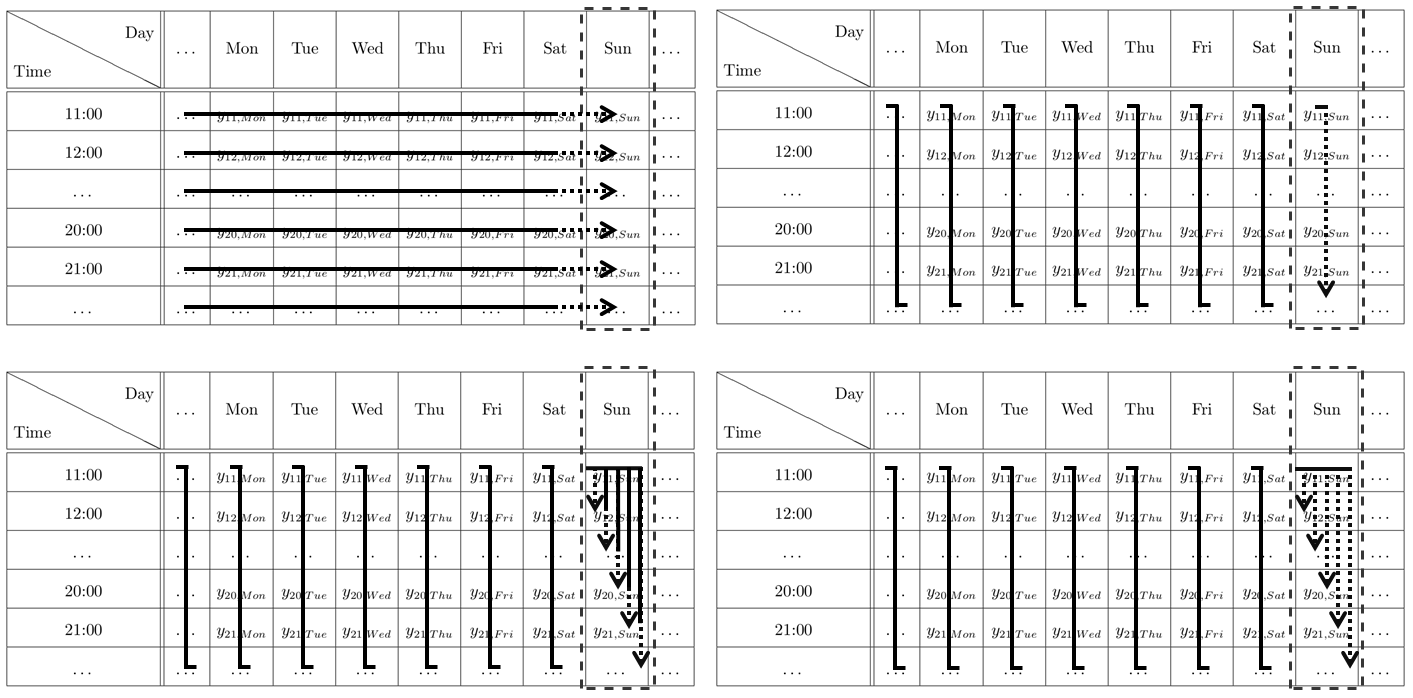
\includegraphics[width=.95\linewidth]{static/model_inputs_gray.png}
\end{center}
